
%!TEX root = thesis.tex
\chapter{Related Works}
\section{Malware Self-Defense}
This section will give an overview of researches about Malware`s self-defense technique, the methods to analyze them, and their application on concurrent architecture. 
This section will try to give the literature about malware evasion techniques. This techniques are generally antonym solution which are found by malware authors, however, there are enough surveys about known technique. We classified all these methods in six categories which are code obfuscation, code reuse, anti debugging, anti emulator and visualization and covert channel over network traffic. This taxonomy is well defined by Jonathan A.P Marpaung, et al \cite{marpaung2012survey}, yet malware authors used them to protect their own properties. 


Code obfuscation was originally  found for protecting intellectual property\cite{balakrishnan2005code}, but It aims to puzzle code`s binary against merely static analysis and disassembling\cite{nachenberg1996understanding}. The first known obfuscation method used encryption in order to hide its content. It was called Cascade which is seen first 1986\cite{you2010malware}. This simple architecture of the obfuscation is called packing\cite{internotsecurityteam}. It involve with two part of binary which are slub part, in order to decipher and encipher.\cite{marpaung2012survey}. Cascade was using simple XOR encryption and that was increasing performance.

Early of the 1990s , oligomorphism and polimorphism started to show up\cite{you2010malware}. The main idea behind them is basicly transforming their slub part in each attempt of encryption process\cite{nachenberg1996understanding}. Today, there are two type of  polymorphic approach to generate different variants of slub.\cite{li2011mechanisms}
\begin{itemize}
  \item Rewriting the code each time from pseudo-code so it differs code synthetically which is actually transformation based obfuscation.
  \item Self-cipher itself different, order of these ciphers and using different keys.
\end{itemize}
One of the other important milestone of polymorphic malware is Mutation Engine(MtE) is writen by a Bulgarian virus Author, called The Dark Avanger. It was automated obfuscation tool which actually considered impossible in those times.\cite{anonymous1}

There are also several methods to prevent unpacking process. These methods are collected carefully by Peter Ferrie \cite{ferrie2008anti}. These methods are especially obstacle for automated analysis.

Compare with polymorphic methods, metamorphic approach is more complicated. It is transformation based method instead of encryption  approach.\cite{konstantinou2008metamorphic} Fundamentally, it produce different codes which doing same blue printed semantic. That just mitigate detection possibility because of lack of static code. 

Network traffic, which malware produce are generally Achilles heel for malware, because they are generally adequately unique traffics to be identified\cite{marpaung2012survey}. They usually cover their overt malicious traffic with covert channel methods.\cite{rutkowska2006rootkits}

Code reuse attacks are strong attacks because they do not inject any code in them as obfuscation methods did. They aim to use legitimate software to evade themselves. There are there well known applied version which are return-into-libc, return oriented programming and Frankenstein.

Return into libc attacks were demonstrated by solar designer in 1997 as a method of bypassing non executable stack to executable libc libraries\cite{designer1997getting}. It's object is to change the "ret" infrastructure argument to the known address possibly libc library(stdio, system, etc). However, this attack is limited with libc libraries, which we improved with return oriented programming. 

Return oriented programming is more flex version of retur-into-libc attack, which is introduced by Shacham in 2007\cite{shacham2007geometry}. Return oriented programming purpose a programming language with small gadgets(instruction bound) which involve all ability of Turing's machine\cite{roemer2012return}. Frankenstein is one of the novel application of return oriented programming by Vishwath Mohan and Kevin W. Hamlen\cite{mohan2012frankenstein}.

Anti debugging and anti emulator methods are really usual for today's malware. The survey of Chen Xu et al. showed us in 2008, majority of 6900 on-the-air malware could evade their self with exhibiting benign behavior in sandboxes, debuggers, and virtual machines.\cite{chen2008towards}. VM and debuggers are most important element of dynamic analysis techniques in autonomous sector, because it must run the file just before it touch the working environment. Yet, it is not that knotty to determine whether working environment is virtual or not. Fuzzing cpu bechmarks and comparing results entropy is a good way to determine virtual machines.\cite{franklin2008remote}

Rootkits are the piece of malicious code which aims to crack integrity of the system state. The idea of the remaining invisible to the system state is traced backed one of the oldest virus "Brain"\cite{martin2008}. It was changing the boot process and activate virus during booting. "Tequila" and "1689" viruses followed "Brain" in 1991 and 1993\cite{Ducklin1991}. There are NTRootkit and HackerDeffender rootkits today. The proper classification of the rootkit are prepared by Adnan Abdakka\cite{Adnan2011}.



\section{Malware analysis methods}

\begin{figure}[h]
    \centering
    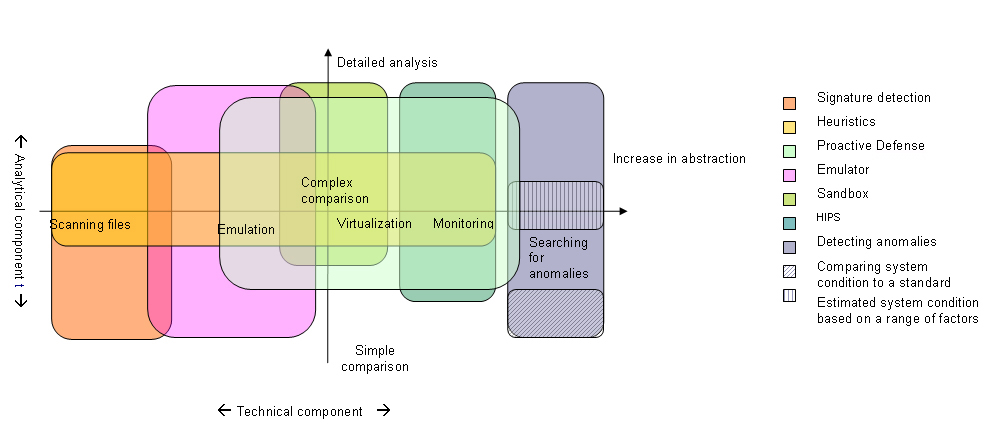
\includegraphics[width=1\textwidth]{img/alisa_1007_pic1_en.jpg}
    \caption{Detection models \cite{Shevchenko2007detc}}
    \label{fig:awesome_image}
\end{figure}
Malware analysis medhods could be considered two dimensional plane which are "anomaly, signature based detection technique" and "Statistic and dynamic analysis method". 



There are also several applied techniques, which combine terminology above. 
\begin{description}
\item[N-gram] It is a anomaly  based heuristic detection method algorithm. It is a bit costly process and not practical for client side analysis. It could be fit for honey pot analysis \cite{reddy2006n} \cite{abou2004n} \cite{abou2004detection}. They are capable against to zero time malwares and that could makes it futures malware detection system. 
\item[Sequential approach on system and funtion call] This approach is anomaly based dynamic analysis and observing and recording the flow graph of systems and function calls and  try to analysis anomaly behaviors.\cite{kendall2007practical}
\item[Taint] It is also called data flow analysis or data flow graph. It is basic tracking marked data values during execution.\cite{saxena2008efficient}\cite{saxena2008efficient}\cite{smith2007principles}
\item[Control Flow Graph] They are one of the most important arm of commercial autonomous malware detection tools\cite{lee2010detecting} \cite{christodorescu2006static} \cite{christodorescu2005semantics}. After the invention of the polymorphic and metamorphic, syntactic analysis could not bear with them. Then we moved to upper layer of information, semantic layer. Semantic can be representation of code flow, and the routes of the code are adequate to produce signature to identify malware. This methods are a member of static analysis and disassembling and source code analysis job.
\item[Network Monitoring] Malware intention of the communication over network actually big clue to detect them. They generally use unique hostname, ip adress or specific protocol with particular way \cite{marpaung2012survey}.
\end{description}